\section{Overenie dát a vyhodnotenie}
\label{sec:results}

Výsledky zahŕňajú kontrolu vstupných súborov, párovanie a klasifikáciu.
Pri každom výsledku sa rozlišuje priamo overená zhoda, experimentálny
kandidát a obmedzenie použitej metódy.

\subsection{Kontrola vybranej vzorky}

Program načítal pôvodný súbor 203~769 vrcholov po častiach a ponechal
časové kroky 20, 29, 30, 32, 35 a 42. Výsledných 28~221 vrcholov je
spojených 31~653 hranami pôvodného grafu. Súčet tried v každom kroku
zodpovedá počtu vrcholov uvedenému v tabuľke~\ref{tab:selected-steps}.

Z vybraných vrcholov má 7~416 známu triedu a 20~805 je neoznačených.
Medzi známymi triedami je 5~981 licitných a 1~435 ilicitných označení.
Obrázok~\ref{fig:selected-distribution} ukazuje výraznú triednu
nevyváženosť aj rozdielnu veľkosť časových krokov. Hodnotenie preto
používa aj metriky zamerané na menej početnú ilicitnú triedu.

\begin{figure}[htbp]
  \centering
  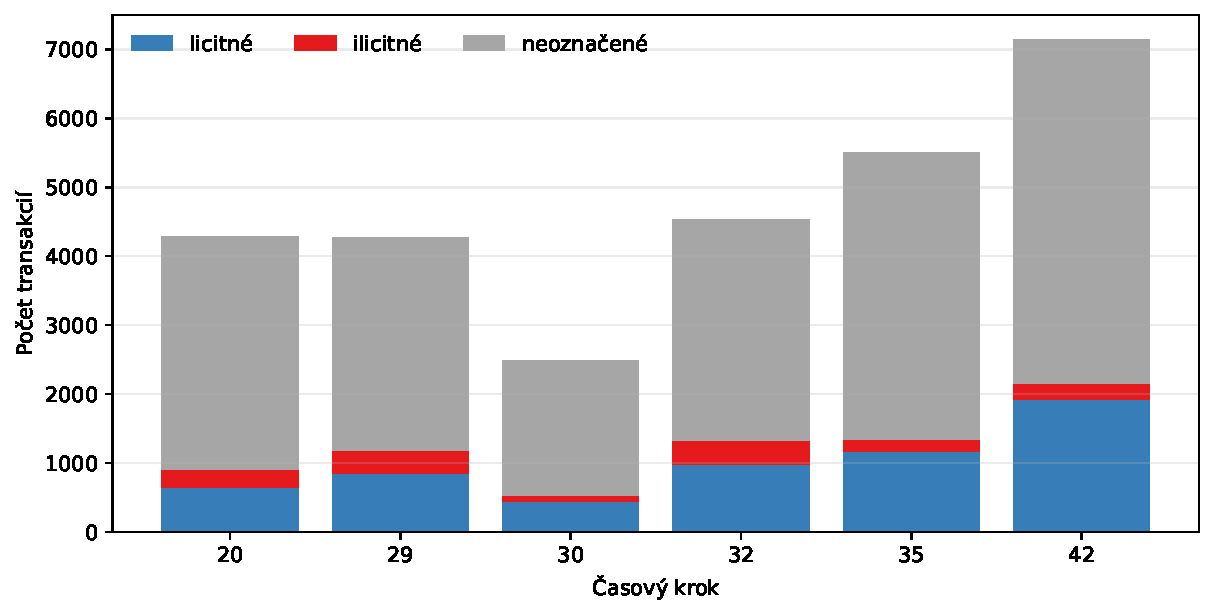
\includegraphics[width=0.9\textwidth]{img/generated/elliptic_class_distribution.pdf}
  \caption{Rozdelenie tried vo vybraných časových krokoch. Vlastné
  spracovanie z pôvodných súborov Elliptic.}
  \label{fig:selected-distribution}
\end{figure}

Verejné mapovanie obsahuje 28~152 z 28~221 vybraných záznamov. Kontrola
formátu overuje, že každý verejný identifikátor má hexadecimálny tvar a
že jeden anonymizovaný identifikátor sa vo výbere nevyskytuje viackrát.
Zvyšných 69 záznamov ostáva bez potvrdeného verejného \texttt{txid}.

\subsection{Kontrola zberu a výpočtu príznakov}

Živá skúška klienta Blockbook overuje načítanie transakcie aj celého
bloku. Pri transakcii sa kontroluje rovnosť medzi poplatkom z odpovede
a rozdielom súčtu vstupov a výstupov, ak sú obe hodnoty dostupné.
Jednotkové testy pokrývajú prevod BTC na satoshi, počet vstupov a
výstupov, jedinečné adresy, coinbase transakciu, rekonštrukciu hrán a
opätovné načítanie odpovede z vyrovnávacej pamäte SQLite.

Ilustračný príklad z obrázka~\ref{fig:utxo-example} má vstupy 0,6 a
0,4 BTC, výstupy 0,8 a 0,19 BTC a vypočítaný poplatok 0,01 BTC. Tento
malý príklad je súčasne testom, že program nezamieňa objem výstupov za
hodnotu vstupov a že poplatok nevytvára ako samostatný výstup.

\subsection{Výsledky párovania}

Z 28~152 známych zhôd bolo vopred skrytých 5~630 záznamov, teda 20~\%
v každom časovom kroku po zaokrúhlení. Množina kandidátov obsahovala
97~533 verejných transakcií zo všetkých 62 zvolených blokov. Správna
transakcia bola pre každý skrytý záznam v dostupnom rozsahu blokov;
počet prípadov bez kandidáta bol preto vo všetkých stupňoch nulový.

\begin{table}[htbp]
  \centering
  \caption{Výsledky párovania na skrytých známych záznamoch. Vlastné
  spracovanie.}
  \label{tab:mapping-results}
  \begin{tabular}{lrrrr}
    \toprule
    Použité príznaky & Top-1 & Top-1 [\%] & Top-5 [\%] & Nejednoznačné \\
    \midrule
    počty vstupov a výstupov & 151 & 2,68 & 5,60 & 5~545 \\
    počty, hodnoty, poplatok a adresy & 5~513 & 97,92 & 99,47 & 166 \\
    všetkých 18 lokálnych príznakov & 5~593 & 99,34 & 99,79 & 50 \\
    \bottomrule
  \end{tabular}
\end{table}

Počty vstupov a výstupov sú slabým identifikátorom, pretože
mnohé transakcie majú rovnakú základnú štruktúru. Po pridaní objemu,
poplatku a jedinečných adries vzrástla top-1 úspešnosť na 97,92~\%.
Úplný lokálny vektor dosiahol 99,34~\%. Zostávajúce kolízie vznikli pri
podobných alebo zhodných vektoroch a pri chybe lineárnej rekonštrukcie.
Pre 69 pôvodne nezmapovaných záznamov sa preto uvádza zoznam kandidátov;
žiadny z nich sa neoznačuje ako potvrdená zhoda.

\begin{figure}[htbp]
  \centering
  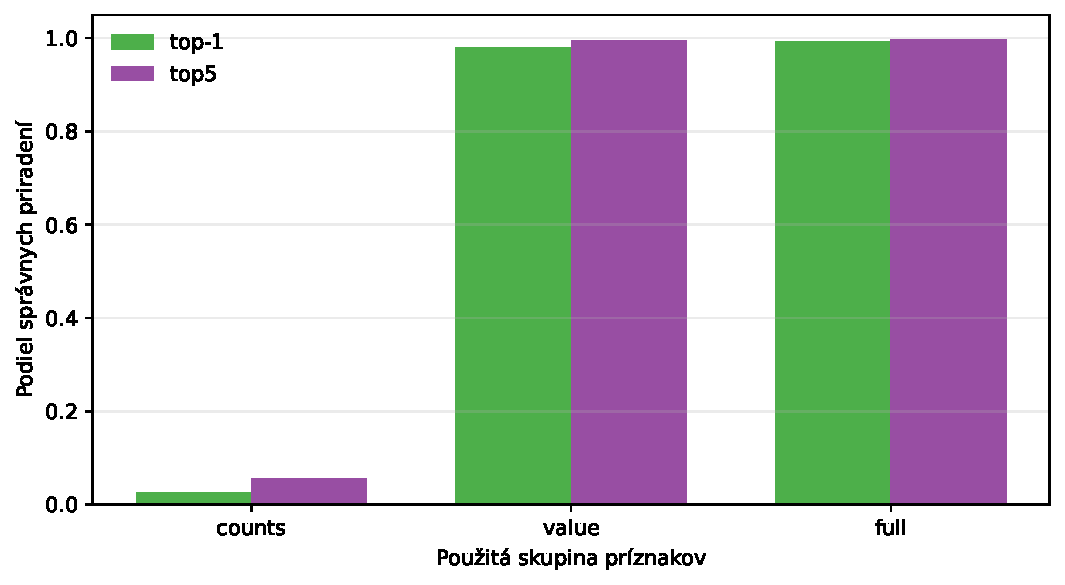
\includegraphics[width=0.82\textwidth]{img/generated/mapping_holdout_accuracy.pdf}
  \caption{Úspešnosť párovania na skrytej časti známych zhôd.
  Vlastné spracovanie.}
  \label{fig:mapping-accuracy}
\end{figure}

\subsection{Porovnanie klasifikačných modelov}

Každá výsledková tabuľka uvádza variant príznakov a grafu,
spôsob rozdelenia, počiatočnú hodnotu generátora, počty označených vrcholov v jednotlivých
častiach a počet použitých hrán. Bez týchto údajov by nebolo možné
rozlíšiť zlepšenie modelu od zmeny experimentálnej vzorky.

Pri náhodnom lese a GCN sa uvádza priemer a smerodajná odchýlka z
piatich počiatočných hodnôt. Logistická regresia je deterministická pri
pevnom vstupe. Rozdiel medzi časovým rozdelením a rozdelením odolným
voči úniku informácií sa
interpretuje spolu s počtom vyradených vrcholov. Pokles $F_1$ po
odstránení spoločných adries môže naznačovať, že pôvodný model využíval
opakované entity. Veľkosť jednotlivých mechanizmov úniku z neho určiť
nemožno.

Po odstránení adresného prekryvu ostalo 8~553 trénovacích, 5~808
validačných a 11~117 testovacích vrcholov. Vyradených bolo 2~743
vrcholov. Rekonštruovaný graf obsahuje 31~586 hrán medzi transakciami
s overeným mapovaním, kým pôvodný graf zvolených krokov obsahuje
31~653 hrán.

Obrázok~\ref{fig:split-retention} ukazuje, v ktorej časti sa počet
vrcholov zmenil. Tréning sa zmenšil iba o 13 nezmapovaných záznamov,
pretože pri prvej časti ešte neexistuje skoršia množina adries, s
ktorou by sa porovnávala. Väčší rozdiel vo validácii a teste vzniká
tým, že neskoršia transakcia sa odstráni, ak opakuje adresu prijatú v
skoršej časti. Graf zobrazuje technické čistenie aj zmenu populácie,
na ktorej sa model hodnotí.

\begin{figure}[htbp]
  \centering
  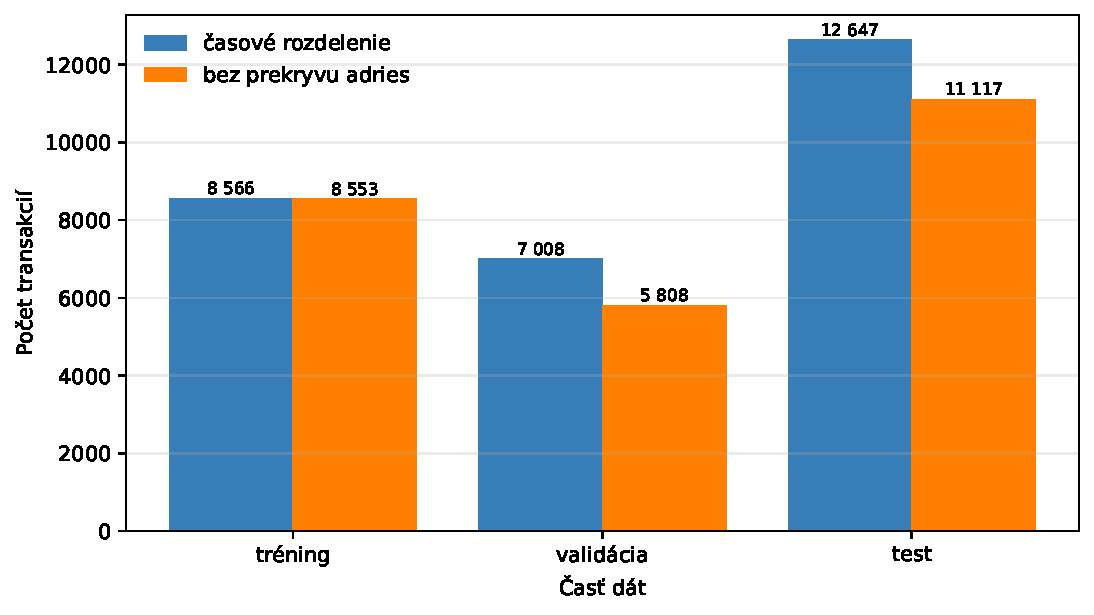
\includegraphics[width=0.82\textwidth]{img/generated/split_retention.pdf}
  \caption{Počet všetkých vrcholov pred odstránením a po odstránení
  pozorovateľného prekryvu adries. Vlastné spracovanie.}
  \label{fig:split-retention}
\end{figure}

Tabuľka~\ref{tab:model-results} uvádza priemernú hodnotu $F_1$ pre
ilicitnú triedu. Skratky A, B a C zodpovedajú variantom definovaným v
kapitole~\ref{sec:methodology}. Pri logistickej regresii sa smerodajná
odchýlka neuvádza, pretože pri pevnom vstupe prebehol jeden
deterministický výpočet.

\begin{table}[htbp]
  \centering
  \caption{Miera $F_1$ ilicitnej triedy; pri RF a GCN priemer
  $\pm$ smerodajná odchýlka z piatich počiatočných hodnôt. Vlastné spracovanie.}
  \label{tab:model-results}
  \begin{tabular}{llcc}
    \toprule
    Variant & Model & Časové rozdelenie & Bez prekryvu adries \\
    \midrule
    A & logistická regresia & 0,602 & 0,593 \\
    A & náhodný les & $0,820\pm0,013$ & $0,881\pm0,003$ \\
    A & GCN & $0,434\pm0,041$ & $0,437\pm0,019$ \\
    \midrule
    B & logistická regresia & 0,483 & 0,494 \\
    B & náhodný les & $0,734\pm0,081$ & $0,625\pm0,120$ \\
    B & GCN & $0,409\pm0,037$ & $0,392\pm0,021$ \\
    \midrule
    C & logistická regresia & 0,483 & 0,494 \\
    C & náhodný les & $0,734\pm0,081$ & $0,625\pm0,120$ \\
    C & GCN & $0,403\pm0,031$ & $0,392\pm0,021$ \\
    \bottomrule
  \end{tabular}
\end{table}

Najvyššiu hodnotu dosiahol náhodný les s pôvodnými príznakmi na
adresne oddelenom teste. Tento výsledok nemožno interpretovať ako
dôkaz, že únik informácií bol odstránený. Variant A stále obsahuje
adresné štatistiky vypočítané k budúcemu bloku 575~059 a oddelený test
má iné zloženie než pôvodný test. Porovnanie opisuje výsledok na
konkrétnej podmnožine; čistý kauzálny účinok jedného zásahu z neho
odvodiť nemožno.

Pri transparentných príznakoch klesol priemerný výsledok náhodného lesa
z 0,734 na 0,625 a variabilita medzi počiatočnými hodnotami vzrástla. Transparentný
vektor obsahuje 18 vlastností bez globálnej histórie adries.
Rozdiel oproti variantu A preto môže súvisieť súčasne s menším počtom
príznakov, odstránením budúcej informácie aj zmenou vzorky. Z tohto
experimentu nemožno tieto tri vplyvy číselne oddeliť.

Výsledky B a C sú pri logistickej regresii a náhodnom lese zhodné, čo
je očakávaná kontrola: tieto modely graf nepoužívajú. Pri časovom
rozdelení sa GCN po rekonštrukcii grafu zmenila z
$0,409\pm0,037$ na $0,403\pm0,031$. Pri adresne oddelenom rozdelení
majú oba grafy 25~619 povolených hrán, a preto poskytli zhodný súhrnný
výsledok $0,392\pm0,021$.

\begin{figure}[htbp]
  \centering
  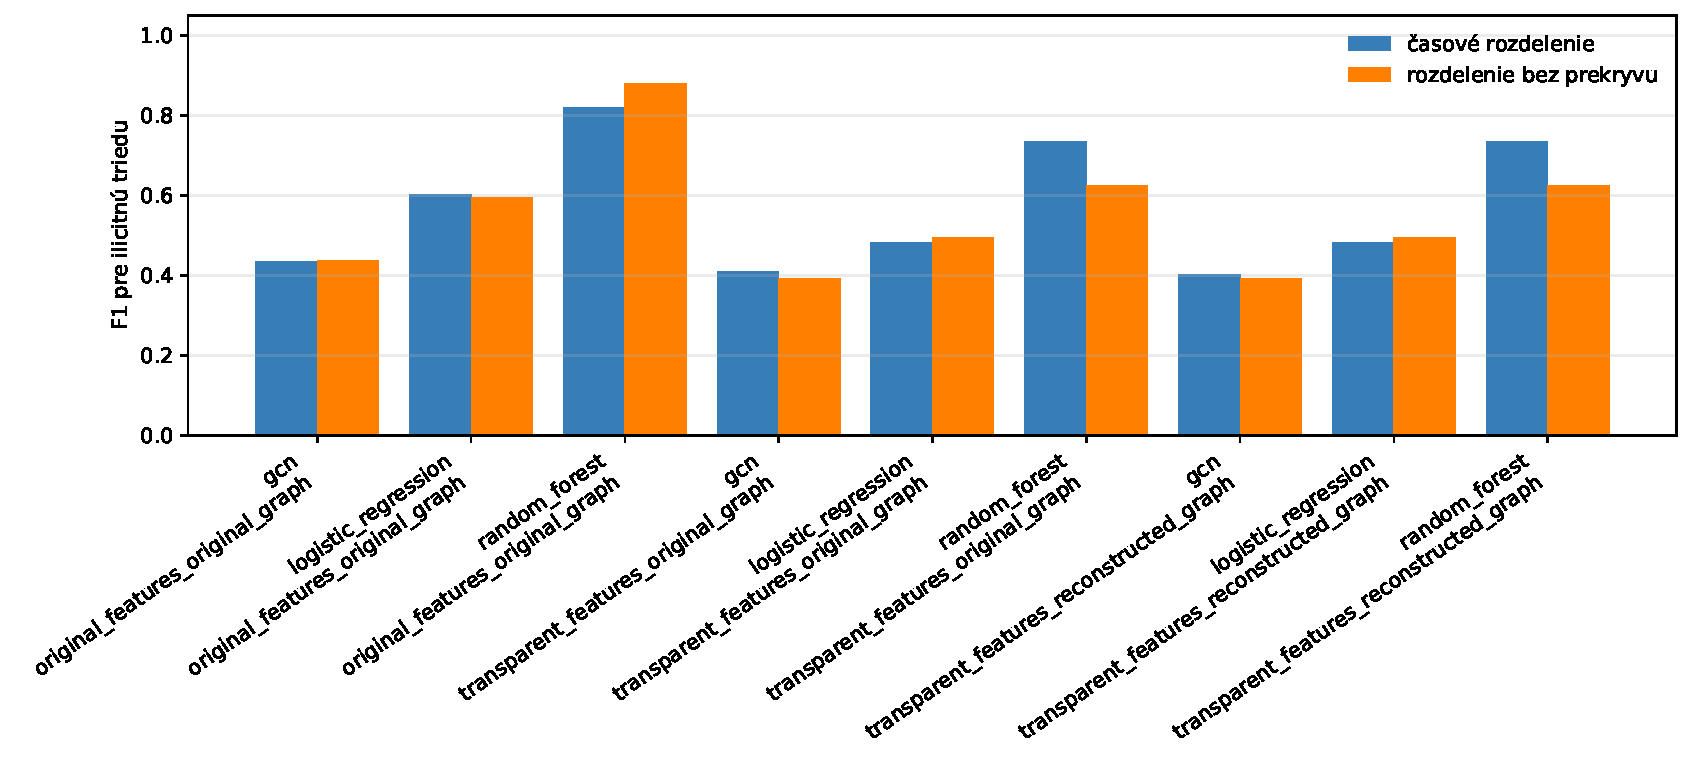
\includegraphics[width=\textwidth]{img/generated/model_f1_leakage_comparison.pdf}
  \caption{Porovnanie $F_1$ ilicitnej triedy pri dvoch spôsoboch
  rozdelenia. Vlastné spracovanie.}
  \label{fig:model-comparison}
\end{figure}

Miera $F_1$ spája precíznosť a úplnosť do jedného čísla. Smer zmeny
medzi väčším počtom upozornení a opatrnejšími predikciami ukazujú obe
zložky osobitne. Obrázok \ref{fig:metric-profile} preto rozkladá výsledok náhodného lesa s
transparentnými príznakmi na päť metrík. Každý stĺpec je priemer z
piatich behov. Precíznosť opisuje čistotu upozornení, úplnosť podiel
zachytených ilicitných označení a PR-AUC poradie skóre pri všetkých
prahoch. Graf tak zabraňuje interpretovať jednu hodnotu $F_1$ bez
informácie o type chýb.

\begin{figure}[htbp]
  \centering
  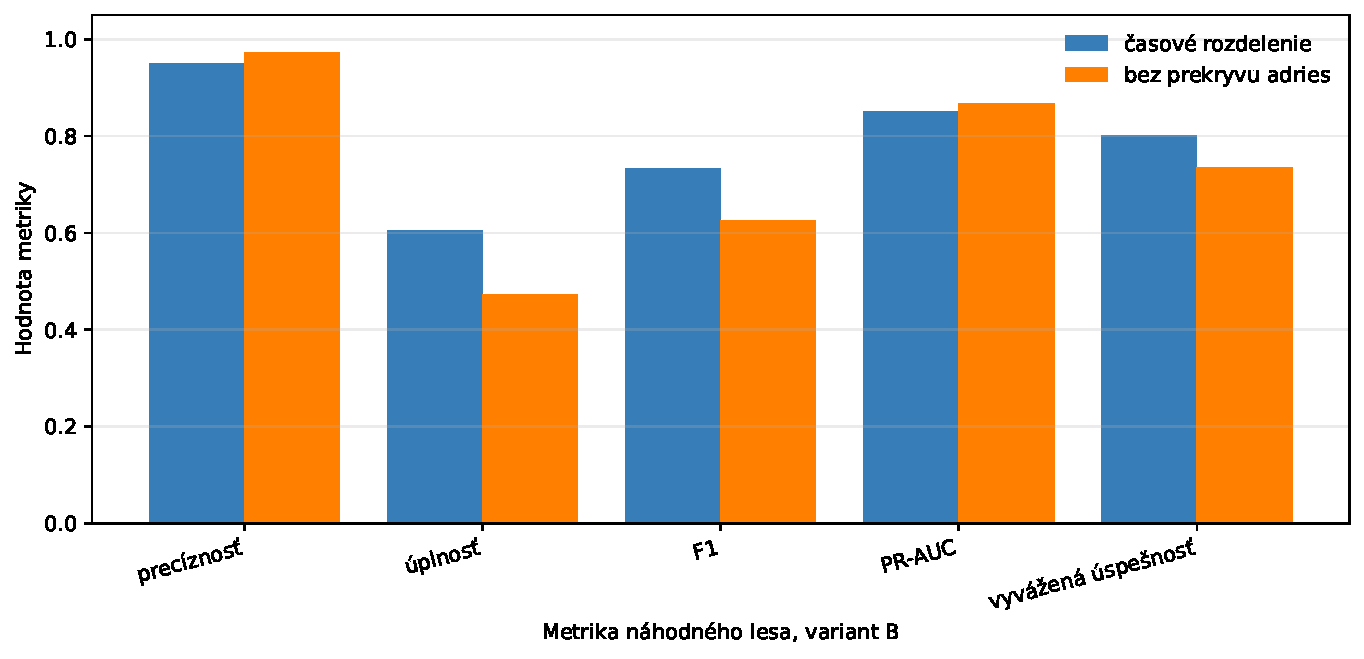
\includegraphics[width=0.92\textwidth]{img/generated/transparent_rf_metric_profile.pdf}
  \caption{Profil metrík náhodného lesa s transparentnými príznakmi,
  variant B. Stĺpce sú priemery z behov s počiatočnými hodnotami
  42--46. Vlastné
  spracovanie.}
  \label{fig:metric-profile}
\end{figure}

\begin{figure}[htbp]
  \centering
  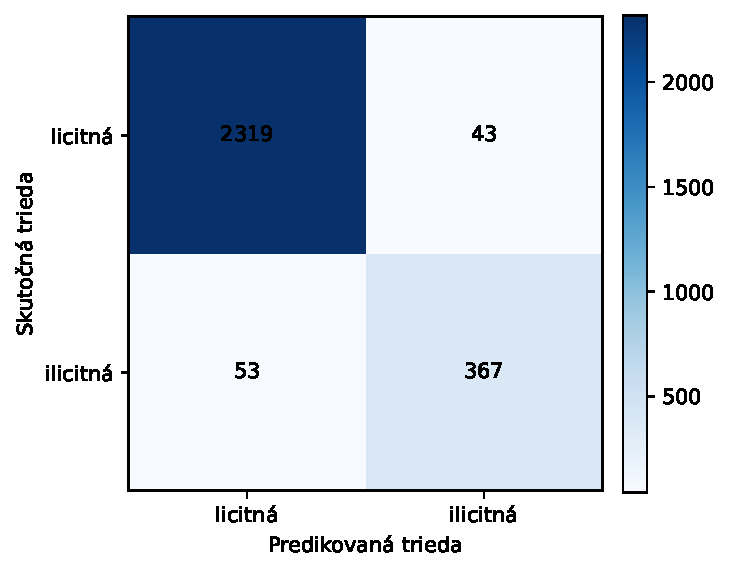
\includegraphics[width=0.55\textwidth]{img/generated/best_model_confusion_matrix.pdf}
  \caption{Matica zámen najlepšieho jednotlivého behu: náhodný les,
  variant A, rozdelenie bez prekryvu adries, počiatočná hodnota 45.
  Vlastné spracovanie.}
  \label{fig:confusion-matrix}
\end{figure}

\subsection{Hrozby pre platnosť}

Prvou hrozbou je správnosť verejného mapovania. Experiment so skrytou
kontrolnou časťou overuje schopnosť zopakovať známe zhody. Pôvod
každého riadka mapovania tým neoveruje. Druhou hrozbou je verejný Blockbook: server môže zmeniť
verziu alebo dočasne odmietnuť požiadavku. Manifest, vlastná hlavička
klienta a lokálna vyrovnávacia pamäť obmedzujú túto závislosť. Úplné
odstránenie by vyžadovalo vlastný zdroj blockchainových dát.

Treťou hrozbou je obmedzenie na šesť časových krokov. Výsledok nemožno
automaticky zovšeobecniť na celý Elliptic ani na súčasné bitcoinové
transakcie využívajúce novšie typy skriptov. Štvrtou hrozbou sú pôvodné
triedy. Zdrojová atribúcia entít nie je zverejnená, takže experiment
hodnotí reprodukciu tried Elliptic. Legalitu transakcií nezávisle
neurčuje.

Napokon, rozdelenie odolné voči úniku informácií odstraňuje transakcie
so spoločnými adresami. Dve odlišné adresy môžu naďalej patriť rovnakej
osobe. Postup kontroluje pozorovateľný prekryv adries; skutočných
vlastníkov nerozdeľuje.
